\chapter{Data types} \label{ch:Datatypes}
\chapterquote{What matters is to live in the present, live now, for every moment is now. It is your thoughts and acts of the moment that create your future. The outline of your future path already exists, for you created its pattern by your past.}{Sai Baba}

\graphicspath{{Chapters/Datatypes/Figures/}}
\lstinputpath{Codes-Verilog/Chapter-Datatypes/VerilogCodes} %path is defined in mypreamble

\section{Introduction}

In the chapter \ref{ch:OverView}, we used the data-types i.e. `wire' and `reg' to define `1-bit' $\&$ `2-bit' input and output ports and signals. Also, some operators e.g. `and ($\&$)' and `or ($|$)' etc. were discussed. In this chapter, some more information is provided on these topics.

\section{Lexical rules}
Verilog is case sensitive language i.e. upper and lower case letters have different meanings. Also, Verilog is free formatting language (i.e. spaces can be added freely), but we use the python like approach to write the codes, as it is clear and readable. Lastly in Verilog, `$//$' is used for comments; also, multiline comments can written between $/* $ and $*/$. 

\section{Data types}\label{sec:DataType}
Data types can be divided into two groups as follows, 
\begin{enumerate}
	\item \textbf{Net group}: Net group represents the physical connection between components e.g. wire, wand and wor etc. In the tutorials, we will use only one net data type i.e. `wire', which is sufficient to create all types of designs. 
	
	\item \textbf{Variable group}: Variable group represents the storage of values in the design. It is always used for the variables, whose values are assigned inside the `always' block. Also, input port can not be defined as variable group. `reg' and `integer' are the example of variable group, which can be synthesized. We will use only `reg' for designing purpose.   
\end{enumerate}

\section{Number representation}
The number can be represented in various format as follows, 
\begin{enumerate}
	\item {Binary Format} \\
	\textbf{reg[1:0] a = 2'b01;} //  number =  1; size = 2 bit;	\\	
	\textbf{reg[2:0] a = 3'b-1;}  // unsigned number= -1 (in 2's complement form); size = 3 bit;\\
	\item {Decimal Format} \\
	\textbf{reg[3:0] a = 3'd1;}   // number = 1; size =3 bit; \\	
	\textbf{reg[3:0] a = 3'd-1;} // unsigned number = -1 (in 2's complement form); size =3 bit;\\
	\item {Signed Decimal Form}\\
	\textbf{reg[3:0] a = 1;}// signed number = 1; size =32 bit; \\
	\textbf{reg[3:0] a = -1;}// signed number = -1; size =32 bit in 2's complement form; \\
	
	\item For hexadecimal and octal representations use `h' and `o' instead of `b' in binary format.  
\end{enumerate}

\section{Signed numbers}
By default, `reg' and `wire' data type are `unsigned number, whereas `integer' is signed number. Signed number can be defined for `reg' and `wire' by using `signed' keywords i.e. `reg signed' and `wire signed' respectively. 

Also, `signed numbers' can be converted into `unsigned numbers' using `\$unsigned()' keyword e.g. if `a = -3 (i.e. 101 in 2's complement notation)', then `\$unsigned(a)' will be `5 (i.e. value of 101)'. Similarly,  `unsigned numbers' can be converted into `signed numbers' using `\$signed()' keyword. 

\begin{noNumBox}
	Although, numbers can be converted from one form to another, but it should be avoided as it may results in errors which are difficult to find. 
\end{noNumBox}

\section{Operators}\label{sec:opearators}
In this section, various synthesizable operators of Verilog are discussed, which are shown in Table \ref{tbl:verilog_operators}. 

\begin{table}[!h]
	\centering
	\caption{Verilog operators}
	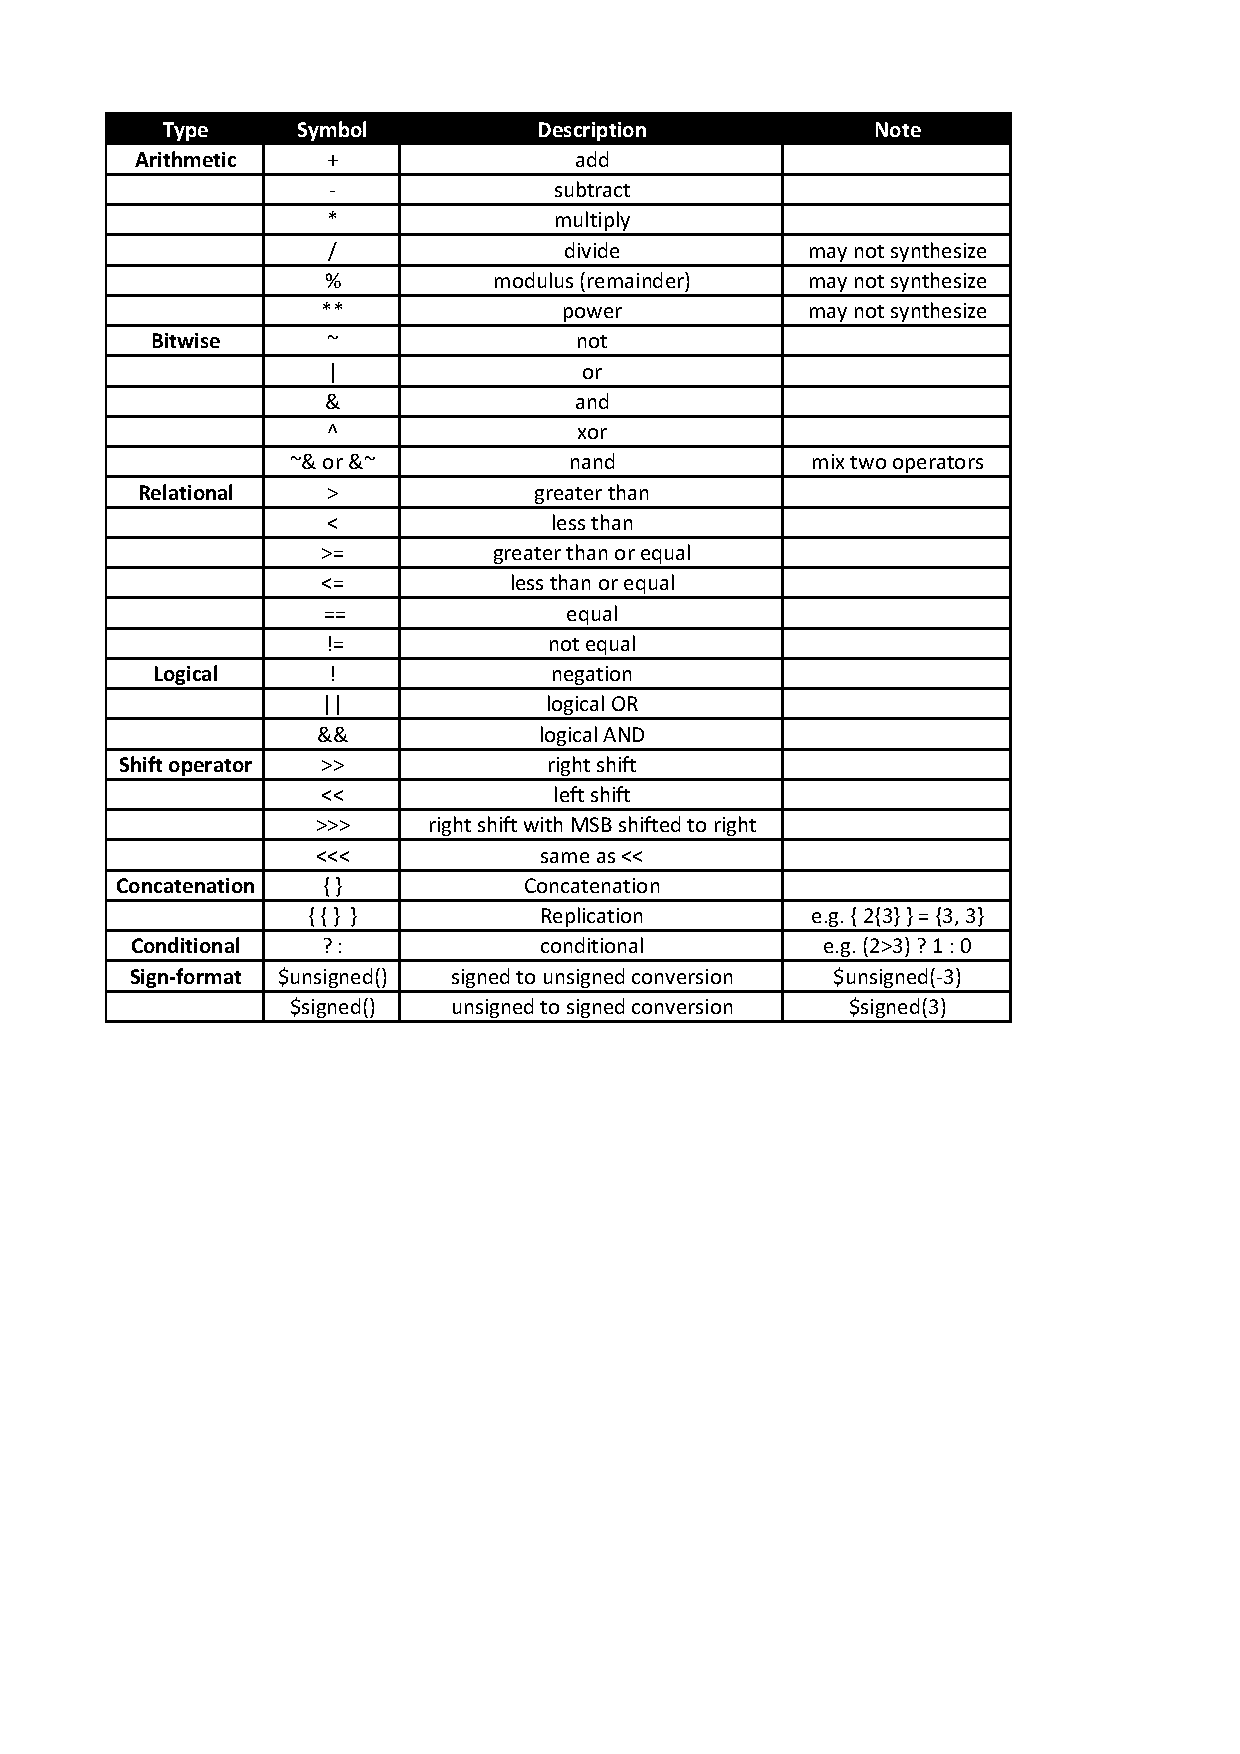
\includegraphics{Verilog_operators}
	\label{tbl:verilog_operators}
\end{table}

\subsection{Arithmetic operator}
Three arithmetic operators i.e. +, -, and * can be synthesized in verilog.

\subsection{Bitwise operators}
Four bitwise operator are available in verilog i.e. `$\&$' (and), `$|$' (or), ` $\hat{}$ ' (xor) and `$\sim$' (not). Further, we can combine these operators to define new operators e.g. `$\sim\&$' or `$\&\sim$' can be used as `nand' operations etc. 

\subsection{Relational operators}
We already see the equality relational operation i.e. `==' in section \ref{sec:proceduralModeling}. Further, five relational operators are defined in verilog i.e. `$>$', `$>=$', `$<$', `$<=$' and `$!$='(not equal to). 

\subsection{Logical operators}
We already see the `and' relational operation i.e. `$\&\&$' in section \ref{sec:proceduralModeling}. Further, three relational operators are defined in verilog i.e. `$||$' (or), `$\&\&$' and `$!$'(negation).

\subsection{Shift operators}
Verilog provides 4 types of shif operators i.e. $>>$, $<<$, $>>>$, $<<<$. Let `a = 1011-0011', then we will have following results with these operators, 
\begin{enumerate}
	\item a $>>$3 = 0001-0110 i.e. shift 3 bits to right and \textbf{fill the MSB with zeros}. 
	\item a $<<$ 3 = 1001-1000 i.e. shift 3 bits to left and \textbf{fill the LSB with zeros}. 
	\item a $>>>$3 = 1111-0110 i.e. shift 3 bits to right and \textbf{fill the MSB with sign bit} i.e. original MSB. 
	\item a $<<<$3 = 1111-0110 i.e. same as a$<<3$.
\end{enumerate}
\subsection{Concatenation and replication operators}

\textbf{Concatenation operation} `\{ \}' is used to combine smaller arrays to create a large array as shown below, \\ \\
wire[1:0] a = 2b'01;\\
wire[2:0] b = 3b'001;\\
wire[3:0] c ;\\
assign c = \{a, b\} // c = 01001 is created using a and b; \\
\\
\textbf{Replication operator} is used to repeat certain bits as shown below,\\
assign c = \{ 2\{a\}, 1'b0 \} // c = 01010 i.e. a is repeated two times i.e. 01-01

\subsection{Conditional operator}
Conditional operator ($?:$) can be defined as follows, 
\\
\textbf{assign} c = (a$>$b) \textbf{?} a \textbf{:} b; // i.e. c=a if a$>$b; else c=b;
\\ \\
Also, conditional expression can be cascaded as shown in Listing \ref{verilog:conditionalEx}, where 4$\times$1 multiplexer is designed. Multiplexer is a combinational circuit which selects one of the many inputs with selection-lines and direct it to output. Table \ref{tbl:Multiplexer} illustrates the truth table for $4\times 1$ multiplexer. Here `i0 - i3' the input lines, whereas `s0' and `s1' are the selection line. Base on the values of `s0' and `s1', the input is sent to output line, e.g. if s0 and s1 are 0 then i0 will be sent to the output of the multiplexer.  

\begin{table}[!h]
	\centering
	\caption{Truth table of 4$\times$1 multiplexer}
	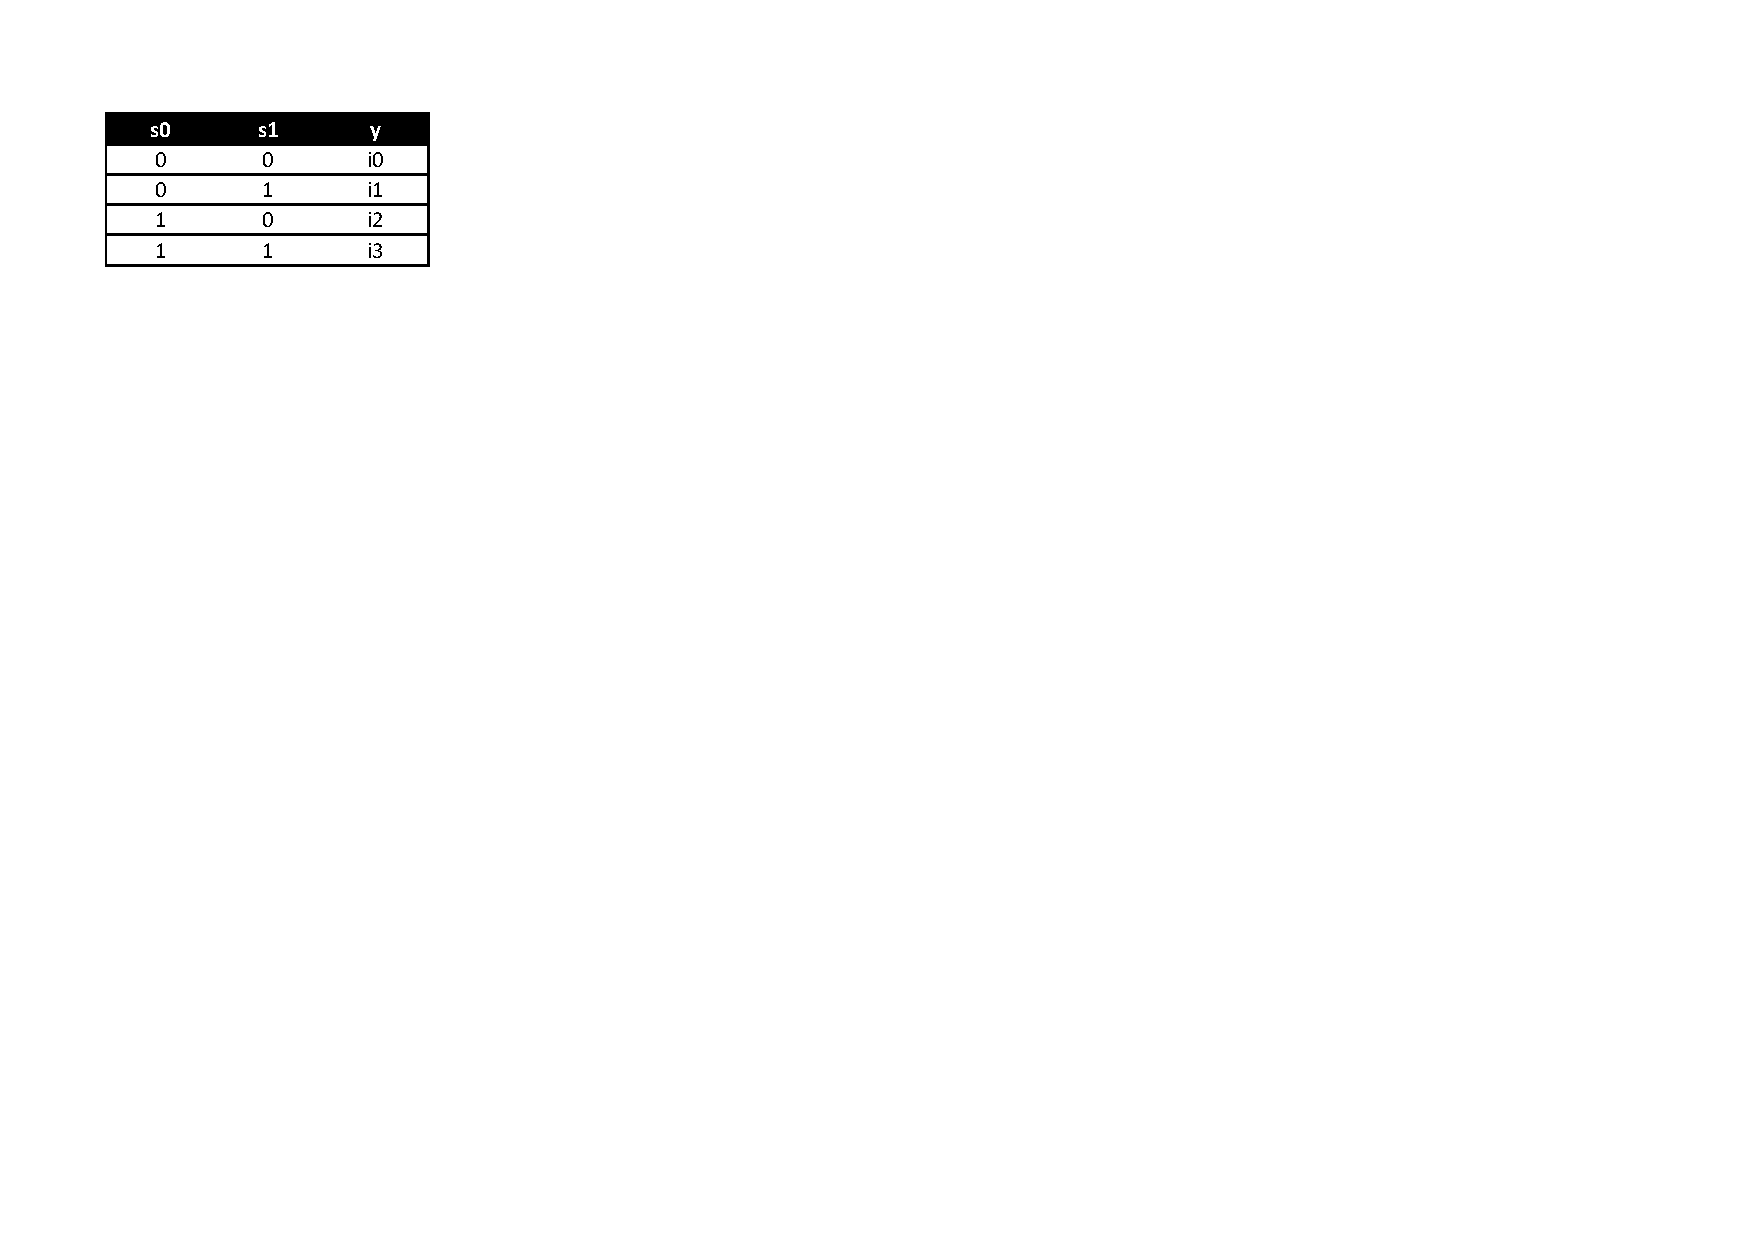
\includegraphics{tableMultiplexer}
	\label{tbl:Multiplexer}
\end{table}

\lstinputlisting[
language = Verilog,
caption    = {Cascaded conditional operator},
label      = {verilog:conditionalEx}
]{conditionalEx.v}

The design generated in Fig. \ref{fig:conditionalEx} is exactly same as the design generated by `if-else statement' which is discussed in Section \ref{sec:ifElse}. Therefore, Fig. \ref{fig:conditionalEx} is described and compared with other designs in Section \ref{sec:ifElse}. Further, Fig. \ref{fig:conditionalExWave} shows the output waveform of the multiplexer which is generated by Listing \ref{verilog:conditionalEx}. 
\begin{figure}
	\centering
	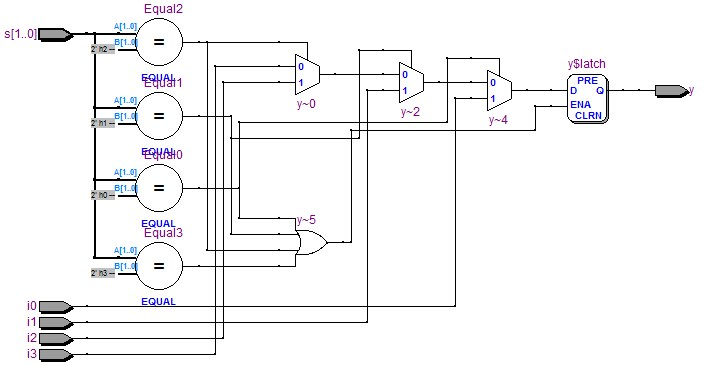
\includegraphics[scale=0.8]{conditionalEx}
	\caption{Multiplexer generated by Listing \ref{verilog:conditionalEx}}
	\label{fig:conditionalEx}
\end{figure}
\begin{figure}
	\centering
	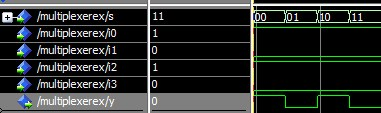
\includegraphics[scale=1]{conditionalExWave}
	\caption{Waveforms of Listing \ref{verilog:conditionalEx}}
	\label{fig:conditionalExWave}
\end{figure}
\section{Parameter and localparam}
Parameter and localparam are used to create reusable codes along with avoiding the `hard literals' from the code as shown in following section. 

\subsection{localparam}
`localparam' keyword is used to defined the constants in verilog. In Listing \ref{verilog:constantEx}, N is defined in line 8 with value 3. Then this value is used in line 10 and 11. Suppose we want to change the constant value to 4. Now, we need to change it only at one place i.e. line 8 (instead of changing everywhere in the code e.g. line 10 and 11 in this example). In this way, we can remove the hard literals from the codes. 

\lstinputlisting[
language = Verilog,
caption    = {Localparam},
label      = {verilog:constantEx}
]{constantEx.v}

\subsection{Parameter and defparam}
`localparam' can not be modified after declaration. But we can define the parameter in the module, which can be modified during component instantiation in structural modeling style as shown below.

\begin{explanation}[Listing \ref{verilog:parameterEx}]
	In line 5, two parameters are defined i.e. `N' and `M'. Then ports `a' and `b' are defined using parameter `N'. The always block (lines 13-19) compares `a' and `b' and set the value of `z' to 1 if these inputs are equal, otherwise set `z' to 0. 
\end{explanation}


\lstinputlisting[
language = Verilog,
caption    = {Parameter},
label      = {verilog:parameterEx}
]{parameterEx.v}


\begin{explanation}[Listing \ref{verilog:parameterInstantEx} and \ref{verilog:parameterInstantEx2}]
	In line 5, `a' and `b' are defined as 4-bit vector. Structural modeling is used in Line 9, where parameter mapping and port mapping is performed. Note that, in line 16, `$.N(5)$' will override the default value of N i.e. N=2 in Listing \ref{verilog:parameterEx}. Also, parameter `M' is not mapped, therefore default value of M will be used, which is defined in Listing \ref{verilog:parameterEx}. In this way, we can remove `hard literals' from the codes, which enhances the reusability of the designs.
	Value of the parameter `N' can also be set using `\textbf{defparam}' keyword, as shown in Listing \ref{verilog:parameterInstantEx2}.
\end{explanation}

\lstinputlisting[
language = Verilog,
caption    = {Parameter instantiation},
label      = {verilog:parameterInstantEx}
]{parameterInstantEx.v}

\lstinputlisting[
language = Verilog,
caption    = {Parameter instantiation using 'defparam'},
label      = {verilog:parameterInstantEx2}
]{parameterInstantEx2.v}

\section{Conclusion}
In this chapter, we saw various  data types and operators. Further Parameters and localparam are shown which can be useful in creating the reusable designs. 
